\documentclass[11pt,a4paper]{jsarticle}
%
\usepackage{amsmath,amssymb}
\usepackage{bm}
\usepackage{epsbox}
\usepackage[dvipdfmx]{graphicx}
\usepackage{verbatim}
\usepackage{wrapfig}
\usepackage{ascmac}
\usepackage{makeidx}
\usepackage[dvipdfmx]{graphicx}

\usepackage{listings, jlisting}
\usepackage{color}
 
\lstset{
    language=Python,%プログラミング言語によって変える。
    numbers = left,
    numberstyle = {\tiny \emph},
    numbersep = 10pt,
    breaklines = true,
    breakindent = 40pt,
    frame = tlRB,
    frameround = ffft,
    framesep = 3pt,
    rulesep = 1pt,
    rulecolor = {\color{black}},
    rulesepcolor = {\color{black}},
    flexiblecolumns = true,
    keepspaces = false,
    basicstyle = \scriptsize,
    identifierstyle = \itshape\scriptsize,
    commentstyle = \fontfamily{ptm}\selectfont\scriptsize,
    stringstyle = \scshape\scriptsize,
    tabsize = 4, 
 }

%
\setlength{\textwidth}{\fullwidth}
\setlength{\textheight}{40\baselineskip}
\addtolength{\textheight}{\topskip}
\setlength{\voffset}{-0.2in}
\setlength{\topmargin}{0pt}
\setlength{\headheight}{0pt}
\setlength{\headsep}{0pt}
%
\newcommand{\divergence}{\mathrm{div}\,}  %ダイバージェンス
\newcommand{\grad}{\mathrm{grad}\,}  %グラディエント
\newcommand{\rot}{\mathrm{rot}\,}  %ローテーション
%
\title{Scratchプログラムの可視化による類似度推定}
\author{G13908 岩科智彩}
\author{G13924 森下汐美}
\date{平成29年1月31日}
\begin{document}
\maketitle
%
%
\section{はじめに}
近年プログラミング教育の推進に伴い、義務教育化が進んでいる。その中で米国マサチューセッツ工科大学のメディアラボが開発したScratchは無償で提供されているグラフィックプログラミング環境である。プログラミングを行う際の命令を本ツールではブロックを組み合わせて作り上げる。初心者にとっては使いやすい構造となっているため米国では利用が増えているものの、日本のユーザーは全体の1\%にも満たない。そこで実際に本ツールで公表をされているデータを利用してより教育に用いられるツールの解析を目指す。Scratch公式サイトのデータでは全体図の把握が可能であるが1つのプログラムでブロックがどのように使われているか、引用していた場合引用元からどの程度変更させたかは不明である。
従って本研究ではある元のプログラムと関連プログラムのブロックを主に解析し結果を基によりわかりやすいデータ発掘を目指す。
\section{使用した技術}
本研究では2つのプログラムと1つの辞書データを使用する。PPython環境ではjsonモジュールをインポートすることでJSON形式ファイルを読み込み辞書型に変換されるためythonで解析プログラムを作成し、JSON形式でインポートしたScratchプログラムを解析する。
\\ソースコード\ref{saprog}はブロック、スプライトの数、cos類似度を計算結果を出力する。ソースコード\ref{scprog}はcos類似度を実施に計算するプログラムとなっている。cos類似度とはベクトル空間モデルにおいて、文書同士を比較する際に用いられる類似度計算方法である。
\\【数式】
\begin{equation}
\cos(A,B) = \frac{\vec{A} \ast\vec{B}} {|\vec{A}||\vec{B}|}  = \frac{\vec{A}}{|\vec{B}|}\ast\frac{\vec{A}}{|\vec{B}|} = \frac{\sqrt {\sum_{i=1}^{|V|}}}{\sqrt{\sum_{i=1}^{|V|}A_i^2\ast\sum_{i=1}^{|V|}B_i^2}}
\end{equation}
本研究では例”色”に当たる部分を、”ブロックの種類”にして計算を行った。Scratchでは数多くのブロックが用意されており、どのブロックを使用するかによって、まったく異なるプログラムを作成することができる。それぞれのプログラムのブロック数をブロックの辞書(ソースコード\ref{sbprog})に集計をした後、ソートしたものをベクターに直し計算式に適用する。

\section{実験結果}
出力されたデータを用いて散布図に表した。縦軸にcos類似度の値、横軸に出力されたブロック数(スプライト数)を元のプログラム("Pong Starter")の数値で割った値の対数値でとる。数値では(1,1)が最も類似しているプロジェクトであるため似ているものから青、赤、緑、紫、水色で色を区別してプロットをする。

\subsection{ブロック数とcos類似度のグラフ}

\begin{figure}[h]
 \begin{tabular}{cc}
 	\begin{minipage}[t]{0.45\hsize}
	 \centering
	 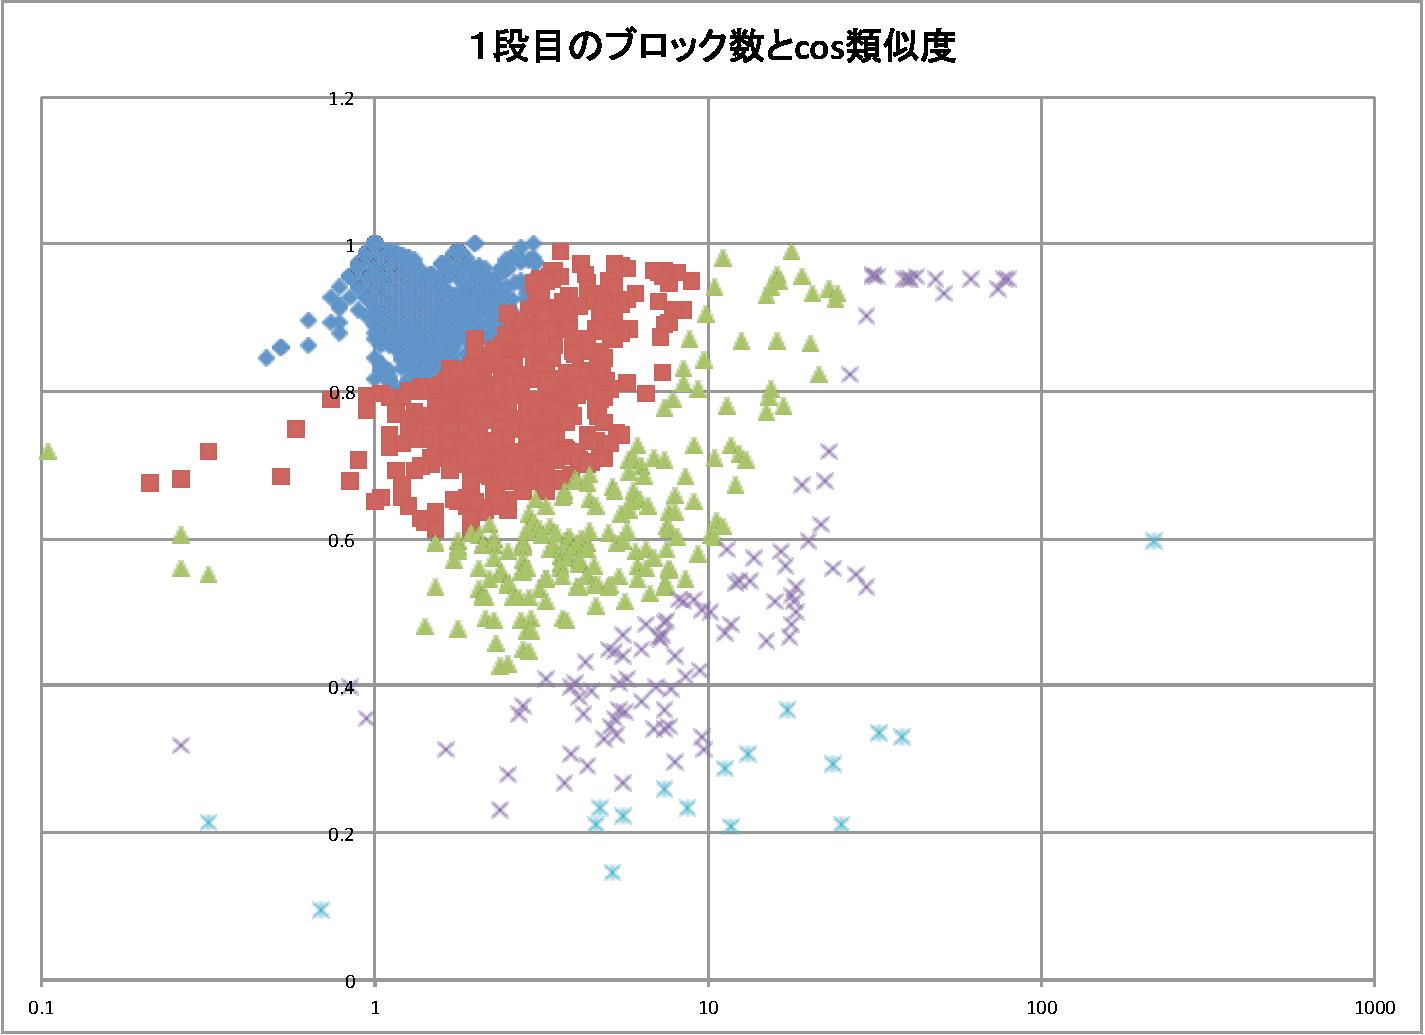
\includegraphics[keepaspectratio, scale = 0.25]{graph_first_block.pdf}
	 \caption{1段目のグラフ}
	 \label{first_block}
	\end{minipage}
        \begin{minipage}[t]{0.45\hsize}
	 \centering
	 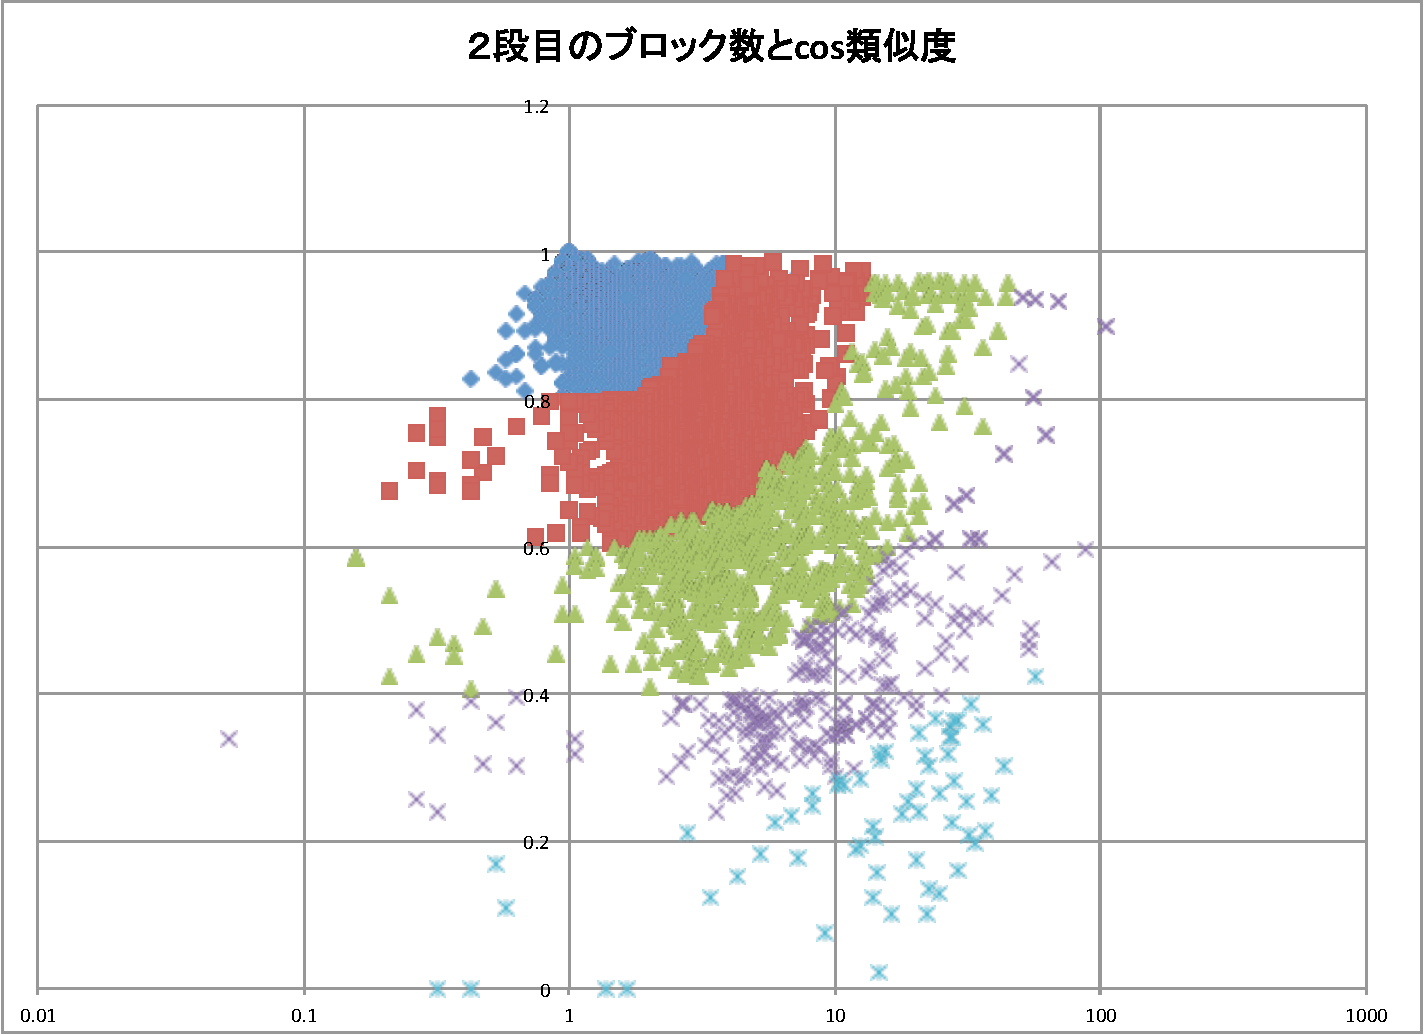
\includegraphics[keepaspectratio, scale = 0.25]{graph_second_block.pdf}
	 \caption{2段目のグラフ}
	 \label{second_block}
	\end{minipage}
 \end{tabular}
  \begin{tabular}{cc}
 	\begin{minipage}[t]{0.45\hsize}
	 \centering
	 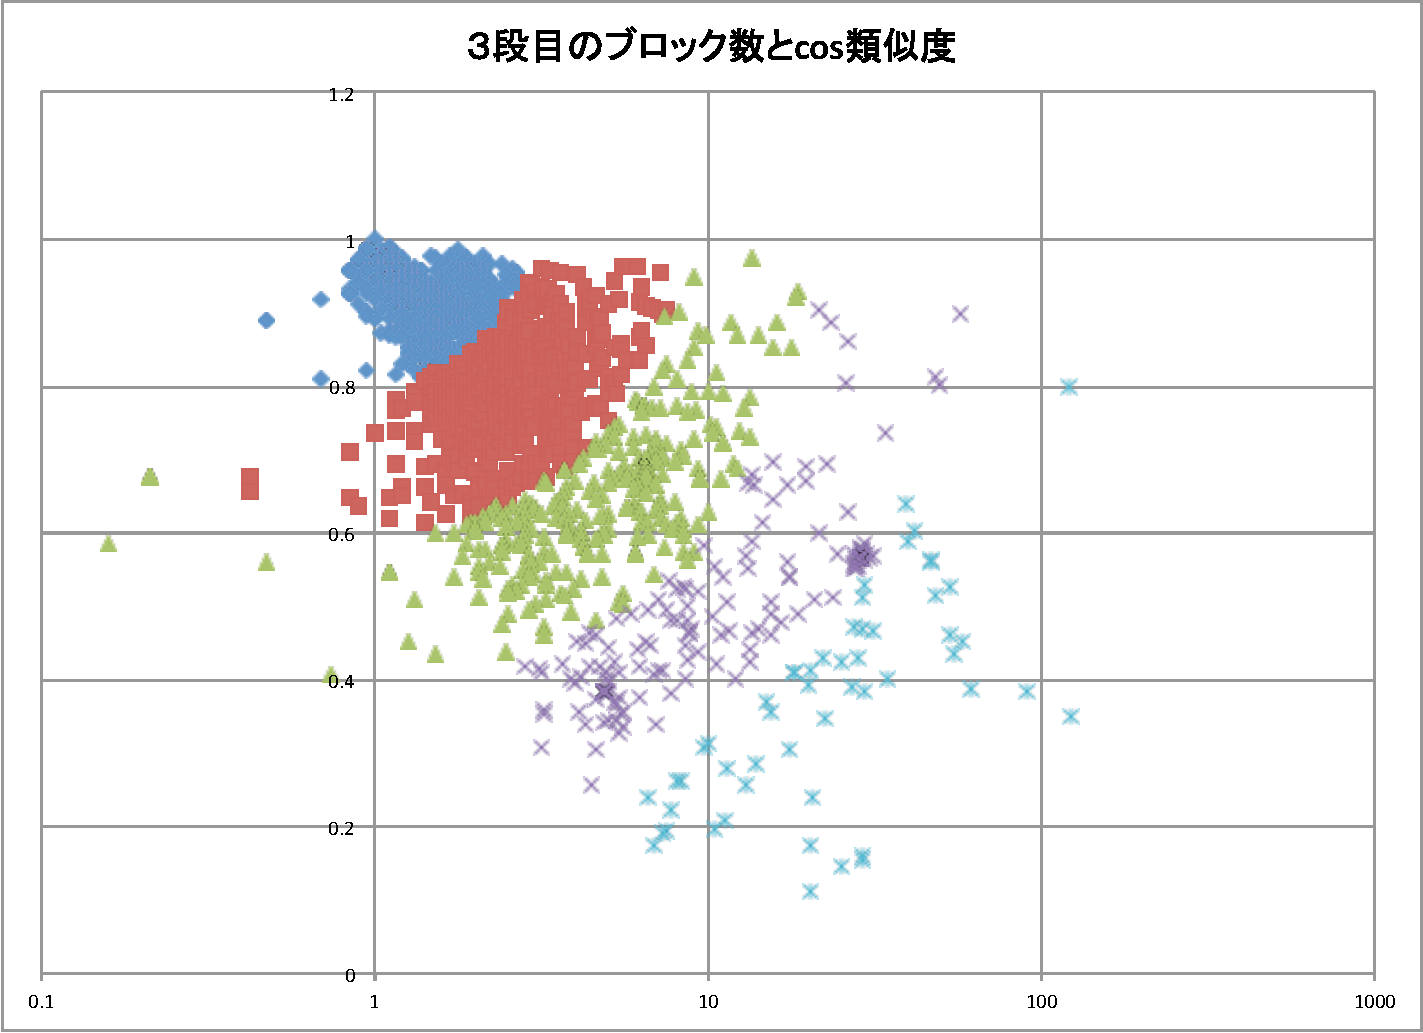
\includegraphics[keepaspectratio, scale = 0.25]{graph_third_block.pdf}
	 \caption{3段目のグラフ}
	 \label{third_block}
	\end{minipage}
        \begin{minipage}[t]{0.45\hsize}
	 \centering
	 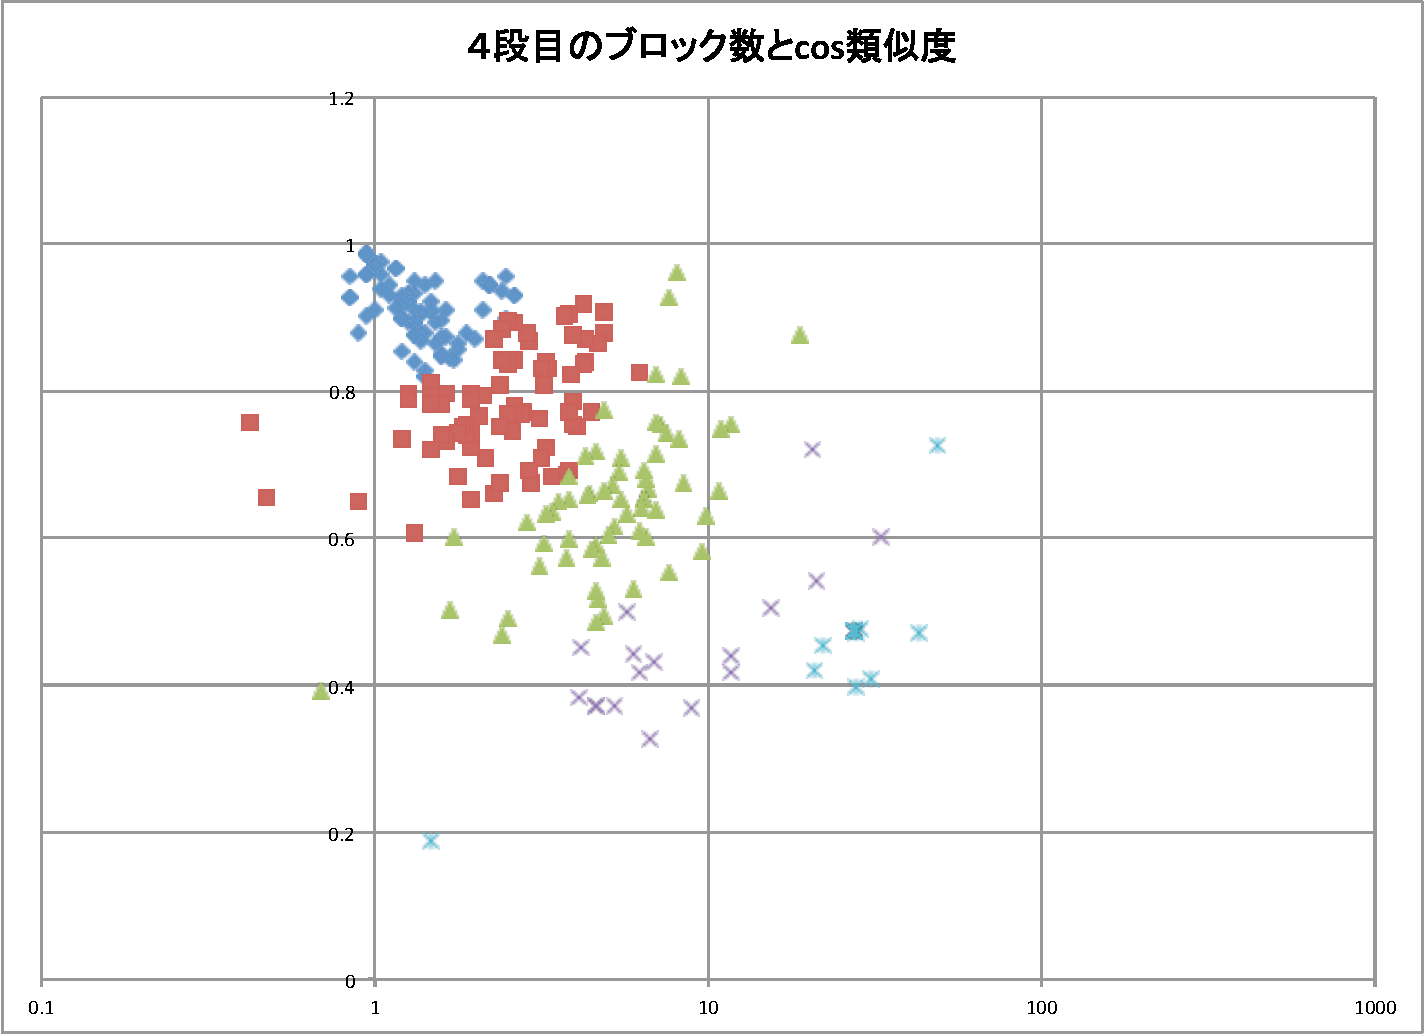
\includegraphics[keepaspectratio, scale = 0.25]{graph_fourth_block.pdf}
	 \caption{4段目のグラフ}
	 \label{fourth_block}
	\end{minipage}
 \end{tabular}
 \end{figure}

\subsection{スプライト数とcos類似度のグラフ}

\begin{figure}[h]
 \begin{tabular}{cc}
 	\begin{minipage}[t]{0.45\hsize}
	 \centering
	 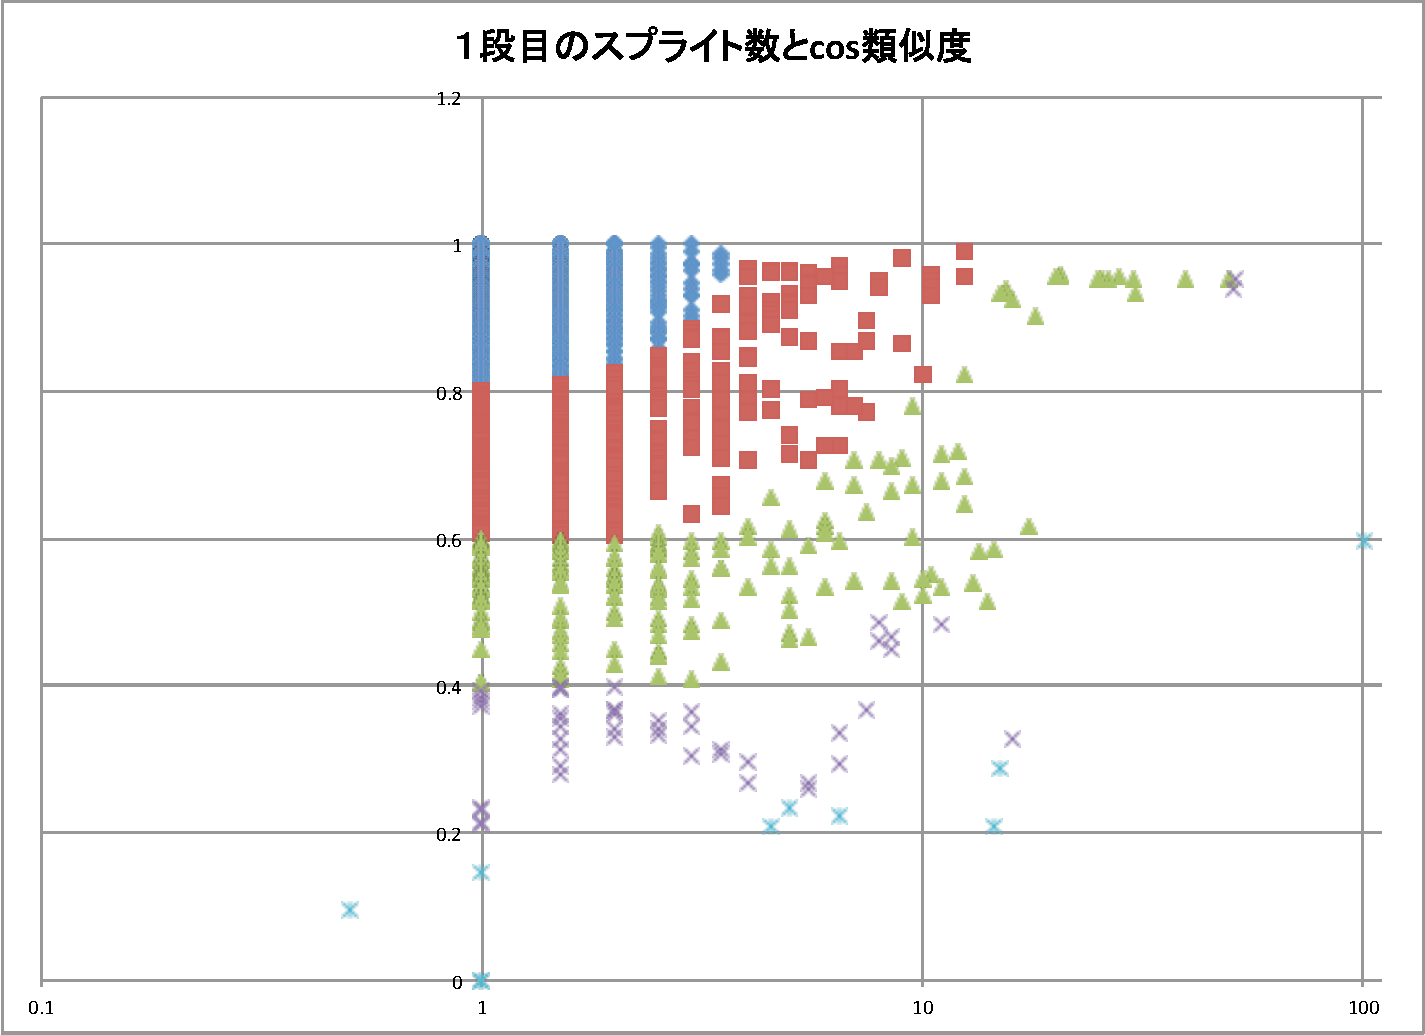
\includegraphics[keepaspectratio, scale = 0.25]{graph_first_splite.pdf}
	 \caption{1段目のグラフ}
	 \label{first_splite}
	\end{minipage}
        \begin{minipage}[t]{0.45\hsize}
	 \centering
	 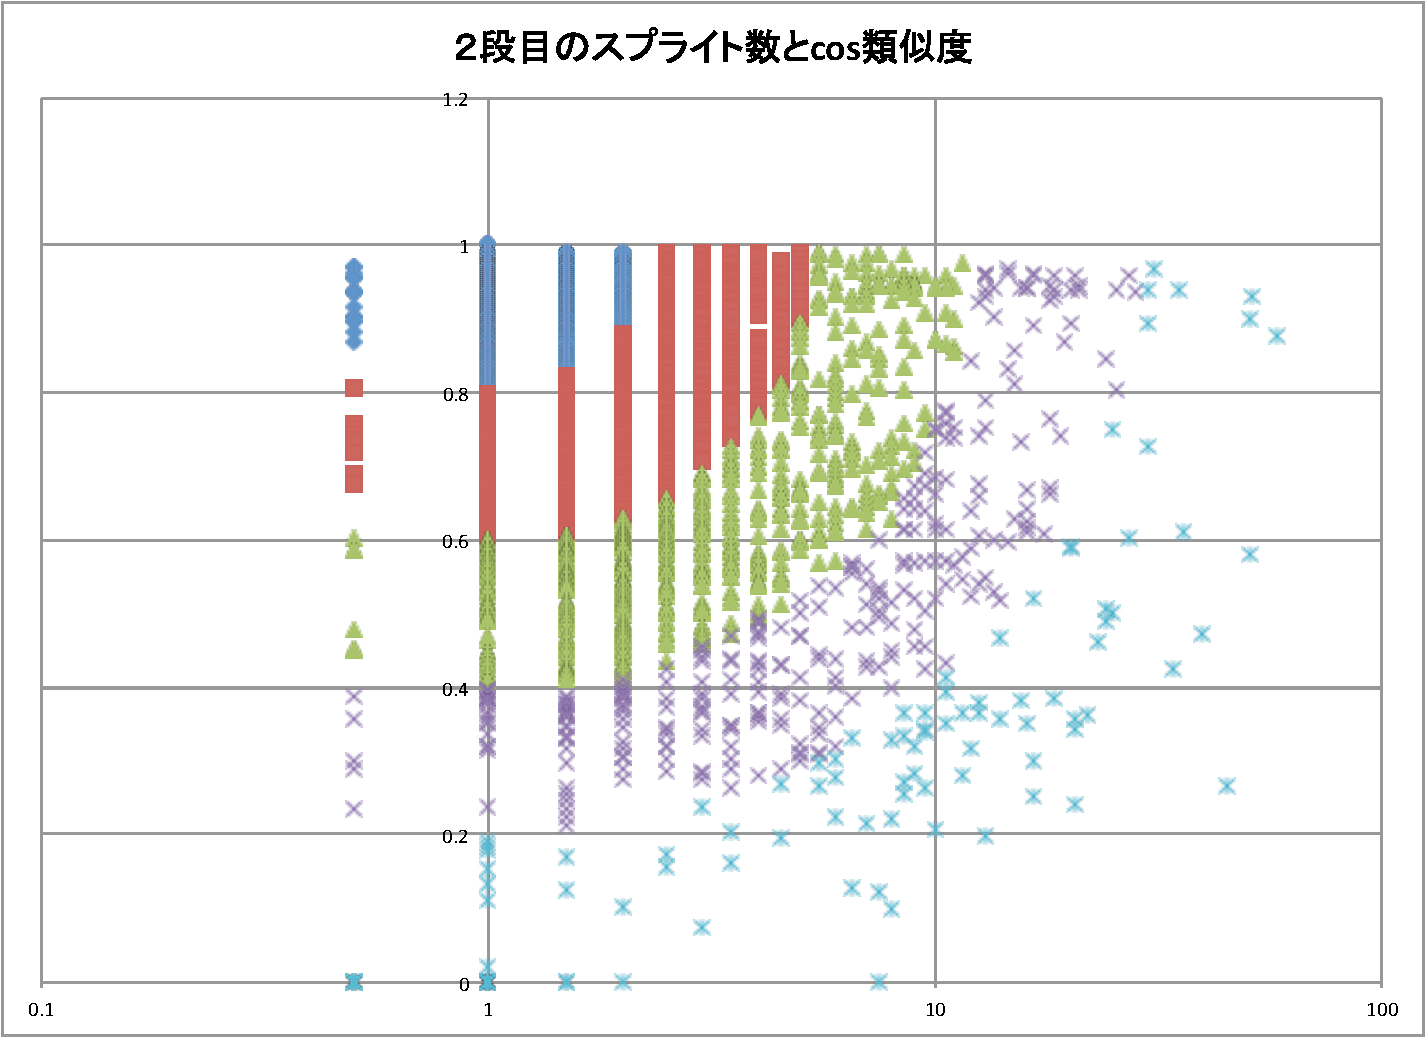
\includegraphics[keepaspectratio, scale = 0.25]{graph_second_splite.pdf}
	 \caption{2段目のグラフ}
	 \label{second_splite}
	\end{minipage}
 \end{tabular}
  \begin{tabular}{cc}
 	\begin{minipage}[t]{0.45\hsize}
	 \centering
	 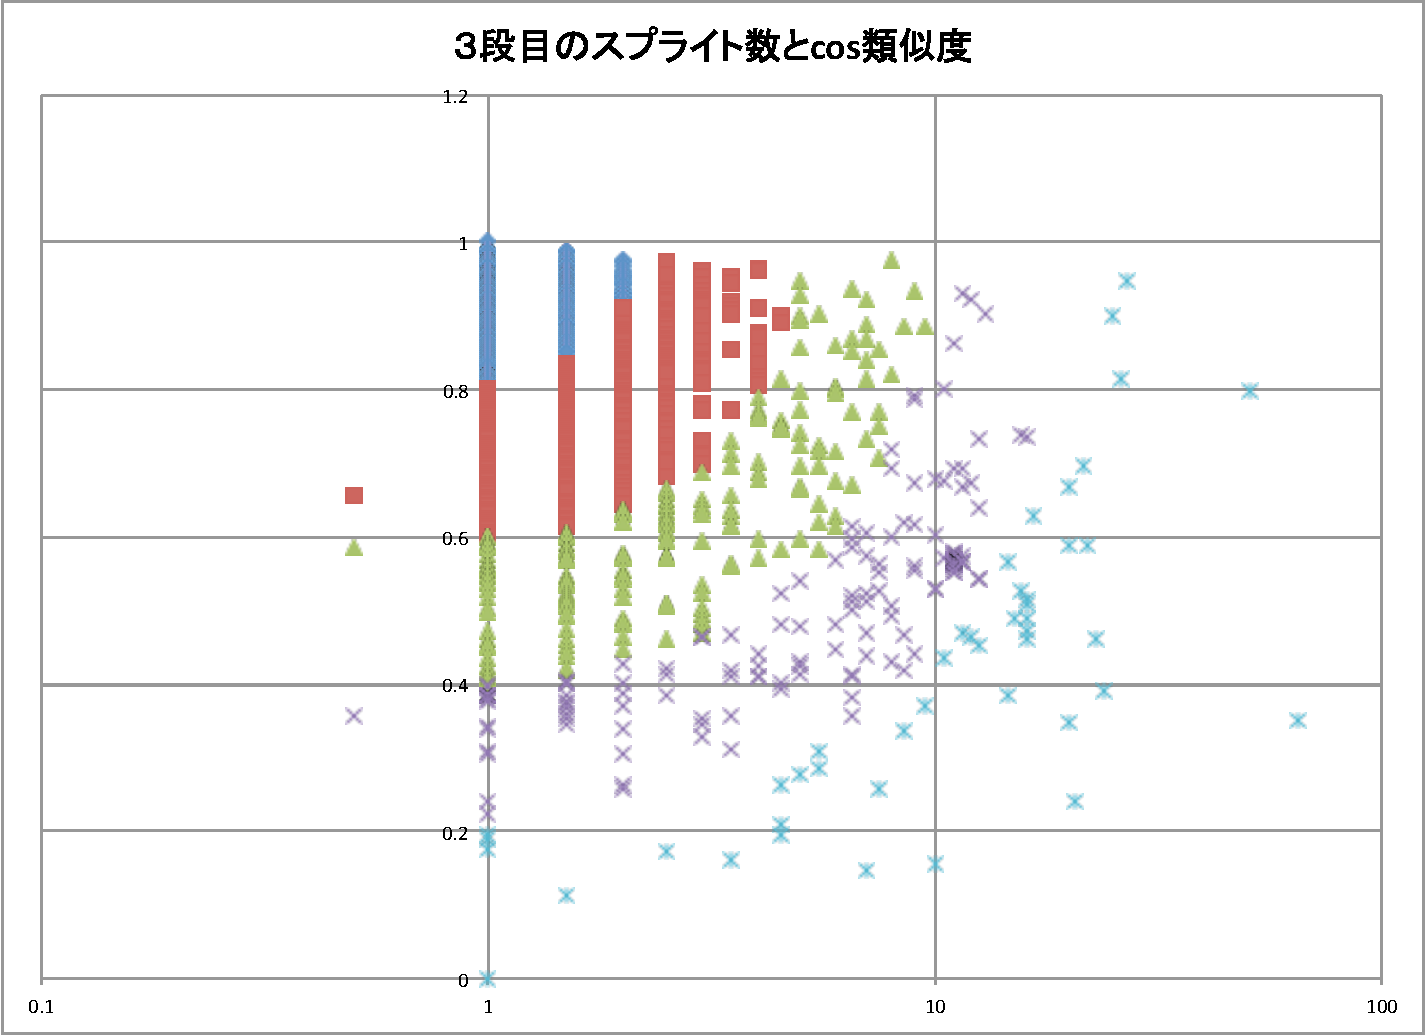
\includegraphics[keepaspectratio, scale = 0.25]{graph_third_splite.pdf}
	 \caption{3段目のグラフ}
	 \label{third_splite}
	\end{minipage}
        \begin{minipage}[t]{0.45\hsize}
	 \centering
	 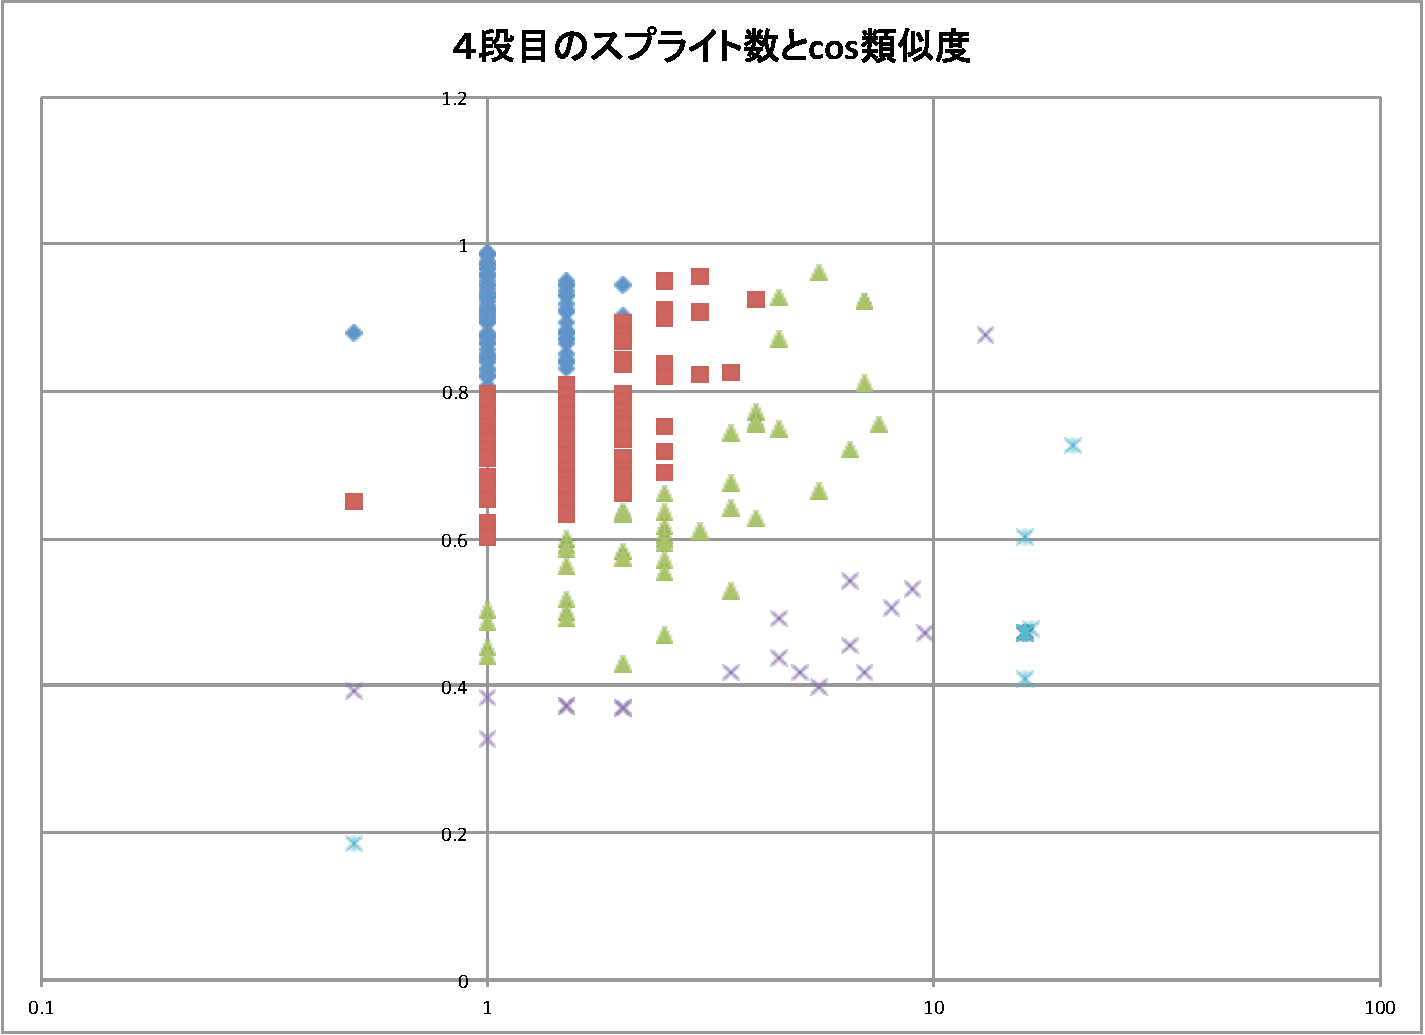
\includegraphics[keepaspectratio, scale = 0.25]{graph_fourth_splite.pdf}
	 \caption{4段目のグラフ}
	 \label{fourth_splite}
	\end{minipage}
 \end{tabular}
 \end{figure}

\newpage 
\section{評価}

\section{まとめ}

\newpage
\lstinputlisting[caption=SimCalculator.py,label=scprog]{SimCalculator.py}
\newpage
\lstinputlisting[caption=scratchAnalysis.py,label=saprog]{scratchAnalysis.py}
\newpage
\lstinputlisting[caption=scratch\_block.py,label=sbprog]{scratch_block.py}
\newpage

%
%
\end{document}
